\documentclass[11pt,letterpaper]{article}

% ── Packages ──────────────────────────────────────────────────────────────────
\usepackage[margin=1.1in]{geometry}
\usepackage{amsmath,amssymb,amsthm}
\usepackage{bm}
\usepackage{graphicx}
\usepackage{xcolor}
\usepackage{booktabs}
\usepackage{array}
\usepackage{hyperref}
\usepackage{enumitem}
\usepackage{tikz}
\usetikzlibrary{arrows.meta,positioning,shapes.geometric,fit,backgrounds}
\usepackage{caption}
\usepackage{subcaption}
\usepackage{float}
\usepackage{microtype}
\usepackage{parskip}
\usepackage{mdframed}
\usepackage{tcolorbox}
\tcbuselibrary{skins,breakable}

% ── Colors ────────────────────────────────────────────────────────────────────
\definecolor{blue1}{RGB}{30,100,180}
\definecolor{green1}{RGB}{30,140,80}
\definecolor{red1}{RGB}{180,40,40}
\definecolor{orange1}{RGB}{200,100,20}
\definecolor{gray1}{RGB}{90,90,90}
\definecolor{boxbg}{RGB}{245,248,255}
\definecolor{boxline}{RGB}{30,100,180}

% ── Hyperref ──────────────────────────────────────────────────────────────────
\hypersetup{
    colorlinks=true,
    linkcolor=blue1,
    citecolor=green1,
    urlcolor=blue1
}

% ── Custom environments ────────────────────────────────────────────────────────
\newtcolorbox{keybox}[1][]{
    enhanced, breakable,
    colback=boxbg, colframe=boxline,
    fonttitle=\bfseries, title=#1,
    left=6pt, right=6pt, top=4pt, bottom=4pt
}
\newtcolorbox{physicbox}[1][]{
    enhanced, breakable,
    colback={RGB}{255,248,235}, colframe=orange1,
    fonttitle=\bfseries\color{orange1}, title=#1,
    left=6pt, right=6pt, top=4pt, bottom=4pt
}

% ── Math macros ───────────────────────────────────────────────────────────────
\newcommand{\R}{\mathbb{R}}
\newcommand{\C}{\mathbb{C}}
\newcommand{\FT}{\mathcal{F}}
\newcommand{\IFT}{\mathcal{F}^{-1}}
\newcommand{\xvec}{\bm{x}}
\newcommand{\kvec}{\bm{k}}
\newcommand{\Geff}{G_{\mathrm{eff}}}
\newcommand{\Gbg}{G_{\mathrm{bg}}}
\newcommand{\Gstar}{G^*}
\newcommand{\eps}{\varepsilon_{\mathrm{latent}}}
\newcommand{\Dsig}{\Delta\sigma}
\newcommand{\aeq}{a_{\mathrm{eq}}}
\newcommand{\norm}[1]{\left\|#1\right\|}

% ──────────────────────────────────────────────────────────────────────────────

\begin{document}

\begin{center}
    {\LARGE\bfseries\color{blue1}
    TSM-FNO: Fourier Neural Operator for\\[4pt]
    Tissue Strain Mapping via MR Elastography}\\[10pt]
    {\large Technical Formulation and Architecture}\\[6pt]
    {\normalsize Eman Richard, Nahil Sobh \quad|\quad \today}
\end{center}

\vspace{-4pt}
\hrule height 1.5pt
\vspace{8pt}

\begin{abstract}
We present \textbf{TSM-FNO}, a Fourier Neural Operator (FNO) that simultaneously predicts the
shear stiffness map $G(\xvec)$, the perilesional latent strain field $\eps(\xvec)$, and the
acoustoelastic constant $A$ from a single 80\,Hz MR Elastography (MRE) acquisition.
This document provides a self-contained derivation of the three physical models underlying
the approach---wave propagation, acoustoelastic pre-stress, and the Lam\'{e} solution for a
pressurized inclusion---followed by a detailed description of the operator learning framework,
network architecture, training procedure, and quantitative results. No prior knowledge of
neural operators or stress-induced anisotropy is assumed.
\end{abstract}

\tableofcontents
\newpage

% ══════════════════════════════════════════════════════════════════════════════
\section{Motivation and Clinical Context}
% ══════════════════════════════════════════════════════════════════════════════

Magnetic Resonance Elastography (MRE) measures the complex shear displacement field
$u(\xvec)$ induced by an external mechanical driver. From $u(\xvec)$ one can infer the local
shear modulus $G(\xvec)$, which encodes tissue stiffness---a marker of fibrosis, tumor, and
neurodegeneration.

In \emph{actively expanding} lesions (e.g., inflating MS lesions or growing tumors), the
internal pressure $p$ generates a radial pre-stress in the surrounding tissue. This
pre-stress modifies the local stiffness through the \emph{acoustoelastic effect}: the same
mechanism by which a tightened drum sounds higher-pitched. The stiffening appears as a
bright ring around the lesion in the stiffness map---a ring that is \emph{absent} in
static, non-expanding lesions.

\textbf{Clinical goal}: distinguish an \emph{expanding} lesion (ring present, $p > 0$) from
a \emph{control} lesion (ring absent, $p = 0$) from a single MRE scan---without requiring
repeated acquisitions or follow-up imaging.

\textbf{Our approach}: train a neural network to invert the MRE wave field directly into
both the stiffness map and the perilesional strain field, in one forward pass, exploiting
the full-image wave context that local inversion methods cannot access.

% ══════════════════════════════════════════════════════════════════════════════
\section{Physical Model}
% ══════════════════════════════════════════════════════════════════════════════

\subsection{Coordinate System and Notation}

We work in a 2-D axial slice of size $N \times N$ voxels at voxel pitch $d_x = 3$\,mm,
giving a field of view of $240 \times 240$\,mm. Physical position is denoted
$\xvec = (x, y)$. All fields are defined on a uniform Cartesian grid.

\subsection{Step 1: Shear Wave Propagation (Helmholtz Equation)}

\subsubsection{Time-Harmonic Form}

In MRE, a pneumatic driver vibrates at a fixed frequency $f = 80$\,Hz. After the
transient has decayed, the tissue oscillates in \emph{steady state}. The displacement at
every point has the form
\[
    \tilde{u}(\xvec, t) = u(\xvec)\,e^{i\omega t}, \quad \omega = 2\pi f.
\]
Substituting into Newton's law for a linear viscoelastic continuum gives the
\textbf{2-D scalar Helmholtz equation}:

\begin{physicbox}[Helmholtz Equation (governing PDE)]
\begin{equation}\label{eq:helmholtz}
    \nabla \cdot \bigl[\Gstar(\xvec)\,\nabla u(\xvec)\bigr]
    + \rho\,\omega^2\, u(\xvec) = 0
\end{equation}
\end{physicbox}

\noindent where:
\begin{itemize}[leftmargin=2em]
    \item $u(\xvec) \in \C$ is the complex shear displacement (Re/Im = amplitude/phase)
    \item $\Gstar(\xvec) = G(\xvec)\bigl(1 + i\xi\bigr)$ is the \emph{complex} shear modulus
    \item $G(\xvec) > 0$ is the storage modulus (stiffness) [Pa]
    \item $\xi = 0.05$ is the loss tangent (viscous damping)
    \item $\rho = 1000$\,kg/m$^3$ is tissue density (assumed uniform)
\end{itemize}

\subsubsection{Why a Complex Modulus?}

Real tissue is \emph{viscoelastic}: it stores energy (elastic, $G$) and dissipates it
(viscous, $\xi G$). The complex modulus $\Gstar = G(1+i\xi)$ captures both.
The imaginary part shifts the phase of the wave. MRE acquires both real and imaginary
parts of $u(\xvec)$, so both components carry stiffness information.

\subsubsection{Finite-Difference Discretization}

Equation~\eqref{eq:helmholtz} is solved numerically by a second-order finite-difference
scheme. At each interior grid node $(i,j)$:

\[
    \frac{G^*_{i+\frac{1}{2},j}(u_{i+1,j} - u_{i,j})
         - G^*_{i-\frac{1}{2},j}(u_{i,j} - u_{i-1,j})}{d_x^2}
    +
    \frac{G^*_{i,j+\frac{1}{2}}(u_{i,j+1} - u_{i,j})
         - G^*_{i,j-\frac{1}{2}}(u_{i,j} - u_{i,j-1})}{d_x^2}
    + \rho\omega^2 u_{i,j} = 0
\]

The half-point moduli use \textbf{harmonic averaging} at material interfaces:
\[
    G^*_{i+\frac{1}{2},j} = \frac{2\,G^*_{i,j}\,G^*_{i+1,j}}{G^*_{i,j} + G^*_{i+1,j}}
\]
Harmonic averaging is physically correct for series-connected springs and prevents the
numerical smearing of sharp stiffness boundaries (e.g., at the lesion edge) that arithmetic
averaging introduces. The resulting sparse linear system $A\bm{u} = \bm{b}$ (size $N^2
\times N^2$) is solved exactly with a direct sparse solver.

\subsubsection{Boundary Conditions}

The domain boundary is driven by $1$--$10$ random complex-amplitude \emph{point sources}
placed on the perimeter. Non-source boundary nodes are set to $u = 0$ (Dirichlet). This
models a pneumatic MRE actuator and ensures the network sees diverse wave patterns during
training.

\subsubsection{Comparison with Murphy ILI}

Murphy et al.\ (2020) use a \emph{Coupled Harmonic Oscillator} (CHO) simulation---a
mass-spring discretization that omits longitudinal wave modes and mode conversion at
material interfaces. Our Helmholtz solver retains these effects, providing more
physically accurate training data at the cost of a denser linear system.

\subsection{Step 2: Acoustoelastic Effect --- Stress-Induced Stiffness Change}

\subsubsection{Physical Mechanism}

When a material is pre-stressed, its elastic moduli change---this is the
\textbf{acoustoelastic effect}. Mechanically, consider a rubber band: under tension it
transmits vibrations faster (higher apparent modulus). In a pressurized lesion, the
surrounding tissue is under circumferential tension (hoop stress), which stiffens it to
shear waves propagating in the radial direction.

\subsubsection{Linear Acoustoelastic Coupling}

To first order in the pre-stress, the effective shear modulus seen by the wave is:

\begin{physicbox}[Acoustoelastic Constitutive Relation]
\begin{equation}\label{eq:acoustoelastic}
    \Geff(\xvec) = \Gbg + A \cdot \Dsig(\xvec)
\end{equation}
\end{physicbox}

\noindent where:
\begin{itemize}[leftmargin=2em]
    \item $\Gbg$ [Pa] --- background stiffness of unstressed tissue
    \item $A$ --- dimensionless acoustoelastic constant (range 2--8 in brain tissue)
    \item $\Dsig(\xvec) = \sigma_{\theta\theta} - \sigma_{rr}$ [Pa] --- deviatoric
          (shear) component of the pre-stress field (difference of hoop and radial stress)
\end{itemize}

\textbf{Why deviatoric stress?} A hydrostatic pre-stress ($\sigma_{rr} = \sigma_{\theta\theta}$)
does not change the resistance to shear. Only the \emph{difference} between stresses in
different directions creates an anisotropic restoring force visible to shear waves.
$\Dsig$ is precisely this shear-relevant component.

\subsubsection{Stress-Induced Anisotropy}

Equation~\eqref{eq:acoustoelastic} describes a \emph{scalar} approximation. In the full
3-D acoustoelastic theory, the effective stiffness tensor $\mathbf{C}_{eff}$ depends on
the direction of wave propagation relative to the principal stress axes:
\[
    C^{eff}_{ijkl} = C^{(0)}_{ijkl} + A_{ijklmn}\,\sigma_{mn}
\]
where $A_{ijklmn}$ is the third-order elastic tensor. For our 2-D scalar shear wave
and a radially symmetric pre-stress, the dominant coupling reduces to
Equation~\eqref{eq:acoustoelastic} with the effective scalar $A$.

\textbf{Implication for imaging}: A shear wave propagating radially outward from an
expanding lesion passes through tissue with non-zero $\Dsig$. It therefore travels
faster (higher $\Geff$) than it would in an unstressed control case. The FNO detects
this speed-up pattern in the complex displacement field.

\subsection{Step 3: Lam\'{e} Solution for a Pressurized Inclusion}

\subsubsection{Setting}

Consider a circular lesion of equivalent radius $\aeq$ (in meters), pressurized at $p$\,Pa,
embedded in an infinite linear-elastic background. This is a classical problem in continuum
mechanics (the \emph{thick-walled cylinder under internal pressure}).

\subsubsection{Analytical Stress Field}

The Lam\'{e} solution gives the radial and circumferential (hoop) stresses at distance $r$
from the lesion center:

\[
    \sigma_{rr}(r) = \begin{cases}
        -p & r \leq \aeq \\[4pt]
        -p\left(\dfrac{\aeq}{r}\right)^2 & r > \aeq
    \end{cases}
    \qquad
    \sigma_{\theta\theta}(r) = \begin{cases}
        +p & r \leq \aeq \\[4pt]
        +p\left(\dfrac{\aeq}{r}\right)^2 & r > \aeq
    \end{cases}
\]

The deviatoric stress is therefore:
\begin{physicbox}[Lam\'{e} Deviatoric Pre-stress]
\begin{equation}\label{eq:lame}
    \Dsig(\xvec) = \sigma_{\theta\theta} - \sigma_{rr} =
    \begin{cases}
        p & r \leq \aeq \quad \text{(inside lesion, uniform compression)} \\[4pt]
        2p\!\left(\dfrac{\aeq}{r}\right)^{\!2} & r > \aeq \quad \text{(outside, decays as } 1/r^2\text{)}
    \end{cases}
\end{equation}
\end{physicbox}

\subsubsection{Physical Interpretation}

Figure~\ref{fig:lame_sketch} illustrates the stress distribution.
Inside the lesion, the pre-stress is uniform---the lesion material is under
equal tension in all directions. Outside, the hoop stress exceeds the
radial stress, creating a differential that stiffens the surrounding tissue to radially
propagating shear waves. The stiffening is strongest at the boundary ($r = \aeq$) and
decays as $1/r^2$, so it is most visible in the \emph{perilesional shell}---a 5\,mm
annulus just outside the lesion boundary.

\begin{figure}[H]
\centering
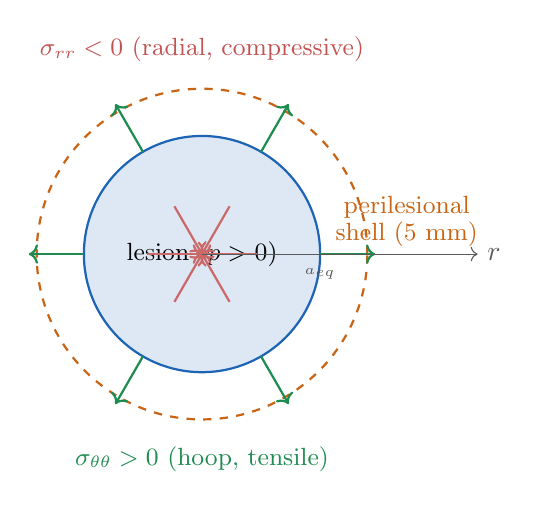
\begin{tikzpicture}[scale=1.0]
    % Lesion circle
    \fill[blue1!15] (0,0) circle (1.5);
    \draw[blue1, thick] (0,0) circle (1.5);
    % Shell
    \draw[orange1, thick, dashed] (0,0) circle (2.1);
    % Labels
    \node at (0,0) {\small lesion ($p > 0$)};
    \node[orange1] at (2.6,0.6) {\small perilesional};
    \node[orange1] at (2.6,0.25) {\small shell (5 mm)};
    % Arrows showing stress
    \foreach \angle in {0,60,120,180,240,300}{
        \draw[->, green1, thick] (\angle:1.5) -- (\angle:2.2);
        \draw[->, red1!70, thick] (\angle:0.7) -- (\angle:0.0);
    }
    % Stress labels
    \node[green1] at (0,-2.6) {\small $\sigma_{\theta\theta} > 0$ (hoop, tensile)};
    \node[red1!80] at (0,2.6) {\small $\sigma_{rr} < 0$ (radial, compressive)};
    % r axis
    \draw[->, gray1] (0,0) -- (3.5,0) node[right] {$r$};
    \node[gray1] at (1.5,-0.25) {\tiny $a_{eq}$};
\end{tikzpicture}
\caption{Stress field around a pressurized circular lesion (Lam\'{e} solution). The
deviatoric stress $\Dsig = \sigma_{\theta\theta} - \sigma_{rr}$ is maximum at the
boundary and decays as $1/r^2$ outside. This differential stress stiffens the tissue to
shear waves, creating the acoustoelastic ring.}
\label{fig:lame_sketch}
\end{figure}

\subsubsection{Ground Truth Labels}

From Equations~\eqref{eq:acoustoelastic} and~\eqref{eq:lame}, the ground-truth
fields used to supervise the FNO are:
\[
    \Geff(\xvec) = \Gbg + A \cdot \Dsig(\xvec), \qquad
    \eps(\xvec) = \frac{\Dsig(\xvec)}{\Gbg}
\]
The latent strain $\eps$ is dimensionless and bounded in $[0, 3]$. It is
\emph{zero everywhere} for a control lesion ($p = 0$), and has a ring-shaped profile
for an expanding lesion. This is the key discriminative signal.

% ══════════════════════════════════════════════════════════════════════════════
\section{The Inverse Problem}
% ══════════════════════════════════════════════════════════════════════════════

\subsection{Forward Problem vs.\ Inverse Problem}

The \textbf{forward problem} is well-posed and has a unique solution:
\[
    \text{Given } G(\xvec),\; \text{solve Eq.~\eqref{eq:helmholtz} to get } u(\xvec).
\]
We use this to \emph{generate training data}: sample random phantom parameters,
compute $\Geff$ via Eq.~\eqref{eq:acoustoelastic}, solve Eq.~\eqref{eq:helmholtz}
for $u$, and store the pair $(u, \Geff, \eps)$.

The \textbf{inverse problem} is what we want to solve clinically:
\[
    \text{Given measured } u(\xvec),\; \text{recover } G(\xvec) \text{ and } \eps(\xvec).
\]
This is \emph{ill-posed}: many stiffness distributions can produce similar wave
fields, especially in the presence of noise. Traditional inversion (direct inversion,
nonlinear inversion) handles ill-posedness through regularization. We handle it
through \emph{supervised learning} on a large synthetic dataset.

\subsection{Why Traditional Inversion Fails at the Ring}

Direct Inversion (DI) computes the local Laplacian of $u$ to estimate $G$ via the
homogeneous Helmholtz equation:
\[
    G = -\frac{\rho\omega^2 u}{\nabla^2 u}
\]
At the lesion boundary, $G$ changes sharply. The Laplacian $\nabla^2 u$ becomes
numerically unstable at discontinuities, requiring spatial smoothing that blurs the
very ring we want to detect. Murphy ILI solves this locally with a 9-voxel CNN
footprint. TSM-FNO solves it globally by learning the full-image operator.

% ══════════════════════════════════════════════════════════════════════════════
\section{From CNN to Neural Operator: The FNO Framework}
% ══════════════════════════════════════════════════════════════════════════════

\subsection{What a CNN Learns (Familiar Ground)}

A convolutional neural network learns a \textbf{function}:
\[
    f_\theta : \R^{C \times H \times W} \to \R^{M}
\]
mapping a fixed-size input (e.g., a $9\times9\times9$ patch) to a fixed-size output
(e.g., one stiffness value). The weights $\theta$ are learned by minimizing a loss
over training examples.

The receptive field is determined by filter size and depth. Larger receptive fields
require deeper networks or larger filters---both expensive.

\subsection{What a Neural Operator Learns (New Concept)}

A \textbf{neural operator} learns to map between \emph{function spaces} rather than
fixed-size vectors:
\[
    \mathcal{G}_\theta : \mathcal{A} \to \mathcal{U}
\]
where $\mathcal{A}$ and $\mathcal{U}$ are spaces of functions defined on a domain
$\Omega \subset \R^2$.

\textbf{Concrete example for MRE}:
\[
    \mathcal{G}_\theta : u(\xvec) \;\longmapsto\; \bigl[G(\xvec),\; \eps(\xvec)\bigr]
\]
The input is the \emph{entire} displacement field $u : \Omega \to \C$; the outputs are
the entire stiffness field $G : \Omega \to \R_{>0}$ and strain field
$\eps : \Omega \to [0,3]$.

\textbf{Key property}: Because the operator is defined on function spaces rather than
finite-dimensional vectors, it is \emph{resolution-invariant}---the same trained
network can in principle operate on finer or coarser grids than used during training.

\subsection{The Fourier Neural Operator (FNO)}

\subsubsection{Core Idea}

The FNO exploits a fundamental identity from Fourier analysis: \emph{convolution in
physical space equals pointwise multiplication in frequency space}. A standard CNN
applies a small spatial filter (limited range). An FNO applies a learned
\emph{global} spectral filter:

\[
    \text{FNO layer:} \quad
    \hat{v}_{\text{out}}(\kvec) = W(\kvec) \cdot \hat{v}_{\text{in}}(\kvec)
    \quad \Leftrightarrow \quad
    v_{\text{out}}(\xvec) = \IFT\bigl[W(\kvec)\,\FT[v_{\text{in}}](\kvec)\bigr](\xvec)
\]

where $\FT$ is the 2-D discrete Fourier transform (DFT), $W(\kvec)$ is a learned
complex weight matrix for each Fourier mode $\kvec$, and $\IFT$ is the inverse DFT.

\textbf{Why this is global}: A single Fourier mode $e^{i\kvec \cdot \xvec}$ spans the
entire domain. Multiplying by $W(\kvec)$ modulates every spatial location simultaneously.
The effective receptive field of one FNO layer is the entire image---not 9 voxels.

\subsubsection{Fourier Block Architecture}

Each of the 4 Fourier blocks in our network performs:

\begin{center}
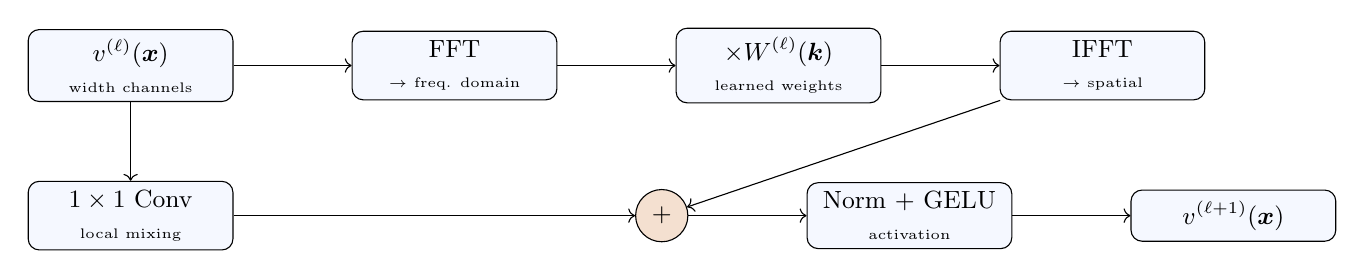
\begin{tikzpicture}[
    node distance=1.4cm,
    box/.style={draw, rounded corners, fill=boxbg, minimum width=2.6cm,
                minimum height=0.65cm, font=\small, align=center},
    op/.style={draw, circle, fill=orange1!20, minimum size=0.55cm, font=\small}
]
    \node[box] (in) {$v^{(\ell)}(\xvec)$\\{\tiny width channels}};
    \node[box, right=1.5cm of in] (fft) {FFT\\{\tiny $\to$ freq. domain}};
    \node[box, right=1.5cm of fft] (mul) {$\times W^{(\ell)}(\kvec)$\\{\tiny learned weights}};
    \node[box, right=1.5cm of mul] (ifft) {IFFT\\{\tiny $\to$ spatial}};
    \node[box, below=1.0cm of in] (conv) {$1\times1$ Conv\\{\tiny local mixing}};
    \node[op, right=5.1cm of conv] (plus) {$+$};
    \node[box, right=1.5cm of plus] (act) {Norm + GELU\\{\tiny activation}};
    \node[box, right=1.5cm of act] (out) {$v^{(\ell+1)}(\xvec)$};

    \draw[->] (in) -- (fft);
    \draw[->] (fft) -- (mul);
    \draw[->] (mul) -- (ifft);
    \draw[->] (ifft) -- (plus);
    \draw[->] (in) -- (conv);
    \draw[->] (conv) -- (plus);
    \draw[->] (plus) -- (act);
    \draw[->] (act) -- (out);
\end{tikzpicture}
\end{center}

The two parallel branches are:
\begin{enumerate}[leftmargin=2em]
    \item \textbf{Spectral branch} (top): FFT $\to$ multiply low-frequency modes by
          learned $W \in \C^{C_{\mathrm{in}} \times C_{\mathrm{out}} \times K_1 \times K_2}$
          $\to$ IFFT. Only the $K_1 \times K_2$ lowest modes are kept
          ($K_1 = K_2 = 16$ in our model). High-frequency modes are zeroed
          (implicit smoothness regularization).
    \item \textbf{Local branch} (bottom): $1\times1$ convolution mixes channels
          independently at each spatial location. No spatial mixing---pure channel
          transformation.
\end{enumerate}
The outputs are added, normalized (InstanceNorm), and passed through GELU activation.
This design ensures both global (spectral) and local (pointwise) information is preserved.

\subsubsection{Why Keep Only Low Modes?}

The stiffness field $G(\xvec)$ and strain field $\eps(\xvec)$ are spatially smooth
(tissue properties vary over centimeters, not millimeters). High-frequency Fourier modes
correspond to fine spatial detail---which in MRE is dominated by noise. Keeping only
16 modes out of 80 available is a form of spectral regularization analogous to
low-pass filtering, but the cutoff frequency and mixing weights are \emph{learned}.

% ══════════════════════════════════════════════════════════════════════════════
\section{TSM-FNO Architecture}
% ══════════════════════════════════════════════════════════════════════════════

\subsection{Input Representation}

The model receives a 4-channel input tensor of shape $(4, N, N)$ with $N = 80$:

\begin{center}
\renewcommand{\arraystretch}{1.3}
\begin{tabular}{cll}
\toprule
Channel & Field & Physical Meaning \\
\midrule
0 & $\mathrm{Re}[u_{80}(\xvec)]$ & In-phase displacement at 80\,Hz \\
1 & $\mathrm{Im}[u_{80}(\xvec)]$ & Quadrature displacement at 80\,Hz \\
2 & $\eps^{\mathrm{prior}}(\xvec) = \Dsig(\xvec)/\Gbg$ & Lam\'{e} pre-stress hint (physics prior) \\
3 & $d(\xvec)/d_{\max}$ & Normalized distance from lesion surface \\
\bottomrule
\end{tabular}
\end{center}

Channels 0--1 are the MRE measurement. Channels 2--3 are \textbf{physics-informed
priors}: channel 2 encodes \emph{where a stiffening ring would appear if the lesion
were expanding} (computed from lesion geometry and an assumed pressure), while channel 3
encodes spatial proximity to the lesion boundary. These priors allow the network to focus
attention on the perilesional region even when the wave signal is noisy.

Additionally, two normalized grid-coordinate channels $x/N$, $y/N \in [0,1]$ are
appended automatically, giving the \textbf{lift layer} an input of $4+2 = 6$ channels.
These grid coordinates break translational symmetry and let the model learn geometry-relative features.

\subsection{Full Network Architecture}

\begin{figure}[H]
\centering
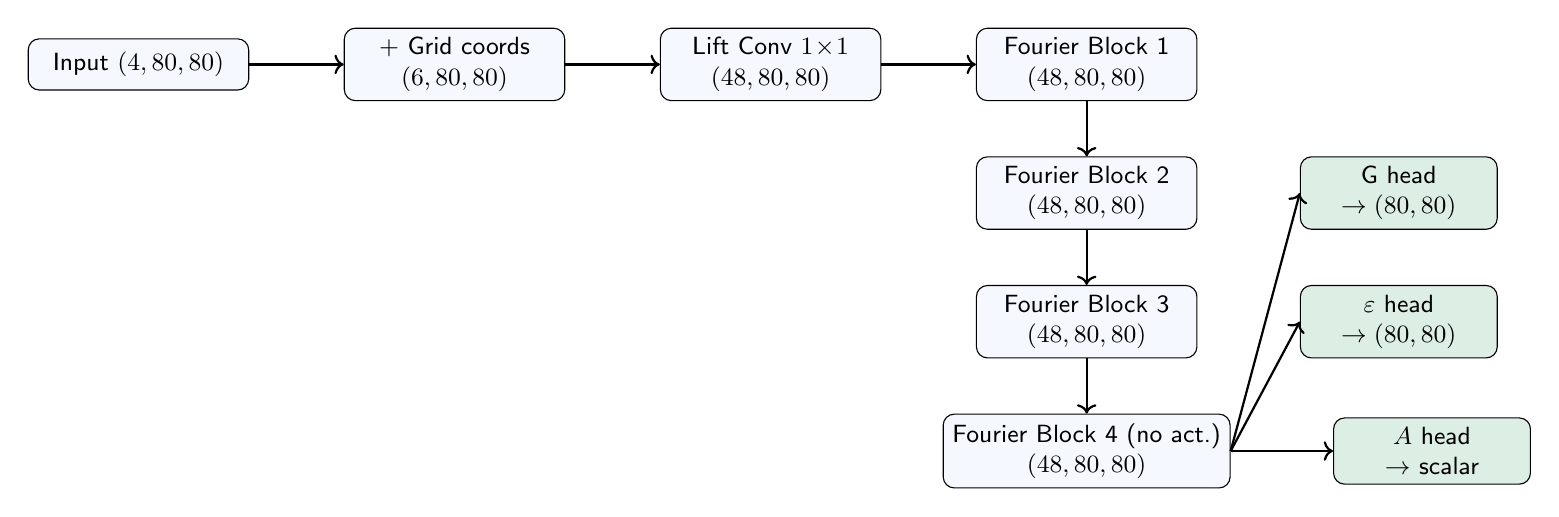
\begin{tikzpicture}[
    node distance=0.9cm and 1.3cm,
    box/.style={draw, rounded corners, fill=boxbg, minimum width=2.8cm,
                minimum height=0.65cm, font=\small\sffamily, align=center},
    head/.style={draw, rounded corners, fill=green1!15, minimum width=2.5cm,
                minimum height=0.65cm, font=\small\sffamily, align=center},
    arr/.style={->, thick}
]
    \node[box] (x) {Input $(4,80,80)$};
    \node[box, right=1.2cm of x] (grid) {$+$ Grid coords\\$(6,80,80)$};
    \node[box, right=1.2cm of grid] (lift) {Lift Conv $1\!\times\!1$\\$(48,80,80)$};

    \node[box, right=1.2cm of lift] (b1) {Fourier Block 1\\$(48,80,80)$};
    \node[box, below=0.7cm of b1] (b2) {Fourier Block 2\\$(48,80,80)$};
    \node[box, below=0.7cm of b2] (b3) {Fourier Block 3\\$(48,80,80)$};
    \node[box, below=0.7cm of b3] (b4) {Fourier Block 4 (no act.)\\$(48,80,80)$};

    \node[head, right=1.3cm of b2] (Ghead) {G head\\$\to(80,80)$};
    \node[head, right=1.3cm of b3] (ehead) {$\varepsilon$ head\\$\to(80,80)$};
    \node[head, right=1.3cm of b4] (ahead) {$A$ head\\$\to$ scalar};

    \draw[arr] (x) -- (grid);
    \draw[arr] (grid) -- (lift);
    \draw[arr] (lift) -- (b1);
    \draw[arr] (b1) -- (b2);
    \draw[arr] (b2) -- (b3);
    \draw[arr] (b3) -- (b4);

    \draw[arr] (b4.east) -- (Ghead.west);
    \draw[arr] (b4.east) -- (ehead.west);
    \draw[arr] (b4.east) -- (ahead.west);
\end{tikzpicture}
\caption{TSM-FNO architecture. The four Fourier blocks process the entire 80$\times$80
feature map simultaneously. Three output heads share the same latent representation.}
\end{figure}

\subsection{Output Heads and Physical Constraints}

Each output head enforces physical bounds through its final activation:

\begin{keybox}[Output Constraints]
\begin{align}
    G(\xvec) &= G_{\min} + (G_{\max} - G_{\min})\cdot\sigma\bigl(h_G(\xvec)\bigr)
    \quad \in [200,\;80{,}000]\;\text{Pa} \label{eq:Ghead} \\[4pt]
    \eps(\xvec) &= \varepsilon_{\max} \cdot \sigma\bigl(h_\varepsilon(\xvec)\bigr)
    \quad \in [0,\;3.0] \label{eq:epshead} \\[4pt]
    A &= -\mathrm{softplus}(h_A) - 2.0
    \quad < -2.0 \label{eq:ahead}
\end{align}
\end{keybox}

where $\sigma(\cdot)$ is the logistic sigmoid, $h_G$, $h_\varepsilon$, $h_A$ are the
raw head outputs, and $\mathrm{softplus}(x) = \log(1 + e^x)$.

\textbf{Why hard bounds?} Without bounded activations, a network might predict
$G = -500$\,Pa (unphysical), $\varepsilon < 0$ (meaningless), or $A = +100$
(outside training distribution). The sigmoid and softplus constraints guarantee
outputs remain physically plausible regardless of the input distribution at test time.

\subsection{Model Size}

\begin{center}
\begin{tabular}{lrl}
\toprule
Component & Parameters & Description \\
\midrule
Lift layer & 288 & $1\times1$ Conv, $6\to48$ channels \\
Fourier Block $\times$4 & 4,718,592 & Spectral weights + bypass conv\\
G head & 12,417 & Conv $48\to128\to1$ \\
$\varepsilon$ head & 3,137 & Conv $48\to64\to1$ \\
$A$ head & 49 & Linear $48\to1$ \\
\midrule
\textbf{Total} & \textbf{4,734,483} & $\approx 18$\,MB at float32 \\
\bottomrule
\end{tabular}
\end{center}

% ══════════════════════════════════════════════════════════════════════════════
\section{Training Procedure}
% ══════════════════════════════════════════════════════════════════════════════

\subsection{Synthetic Dataset Generation}

We generate 50,000 training phantoms. Each phantom is created by:
\begin{enumerate}[leftmargin=2em]
    \item \textbf{Sample geometry}: random elliptical lesion (center, semi-axes, angle)
    \item \textbf{Sample pressure}: $p \in [0, 8000]$\,Pa (20\% control: $p=0$)
    \item \textbf{Sample material}: $\Gbg \in [800, 3000]$\,Pa; $A \in [2, 8]$
    \item \textbf{Compute} $\Geff$ via Eq.~\eqref{eq:acoustoelastic}, $\eps$ via Eq.~\eqref{eq:lame}
    \item \textbf{Solve} Helmholtz (Eq.~\eqref{eq:helmholtz}) for $u_{80}$
    \item \textbf{Assemble input} channels 0--3
    \item \textbf{Add noise}: complex Gaussian, SNR $\in [15, 30]$\,dB
\end{enumerate}

\textbf{Dataset composition} (stratified):
60\% expanding ($p > 0$), 20\% control ($p = 0$), 10\% high-contrast
($G_{\mathrm{lesion}} / \Gbg > 10$), 10\% near-circular geometry.

\subsection{Loss Function}

The total loss is a weighted sum of five physics-motivated terms:

\begin{keybox}[Composite Training Loss]
\begin{equation}\label{eq:loss}
    \mathcal{L} = \underbrace{\mathcal{L}_G}_{\text{stiffness}}
    + \lambda_\varepsilon\,\underbrace{\mathcal{L}_\varepsilon}_{\text{strain MSE}}
    + \lambda_{\mathrm{ring}}\,\underbrace{\mathcal{L}_{\mathrm{ring}}}_{\text{perilesional RL}^2}
    + \lambda_{\mathrm{expand}}\,\underbrace{\mathcal{L}_{\mathrm{expand}}}_{\text{classifier}}
\end{equation}
\end{keybox}

with default weights $\lambda_\varepsilon = 1.0$, $\lambda_{\mathrm{ring}} = 0.5$,
$\lambda_{\mathrm{expand}} = 0.2$. Each term is defined as:

\begin{align*}
    \mathcal{L}_G &= \frac{\norm{G_{\mathrm{pred}} - G_{\mathrm{true}}}^2}{\norm{G_{\mathrm{true}}}^2} \quad \text{(relative $L^2$)} \\[6pt]
    \mathcal{L}_\varepsilon &= \frac{1}{N^2}\sum_{\xvec}\bigl(\eps_{\mathrm{pred}}(\xvec) - \eps_{\mathrm{true}}(\xvec)\bigr)^2 \quad \text{(MSE; stable for zero-target controls)} \\[6pt]
    \mathcal{L}_{\mathrm{ring}} &= \frac{\norm{(\eps_{\mathrm{pred}} - \eps_{\mathrm{true}}) \odot M_{\mathrm{ring}}}^2}{\norm{\eps_{\mathrm{true}} \odot M_{\mathrm{ring}}}^2 + \delta} \quad \text{(relative $L^2$ in shell)} \\[6pt]
    \mathcal{L}_{\mathrm{expand}} &= \mathrm{BCE}\!\left(\;\hat{y},\; \mathbf{1}\left[\max_{\xvec \in M_{\mathrm{ring}}} \eps_{\mathrm{true}}(\xvec) > \theta\right]\right) \quad \text{(binary cross-entropy)}
\end{align*}

where $M_{\mathrm{ring}}$ is the perilesional shell mask (5\,mm annulus), $\delta = 10^{-6}$
prevents division by zero for control samples, and $\hat{y}$ is the network's expansion
prediction $\max(\eps_{\mathrm{pred}}$ in ring$)$.

\textbf{Design rationale for $\mathcal{L}_{\mathrm{ring}}$}: The ring occupies only
$\sim$3\% of the image area. Without the ring-specific loss term, the network minimizes
global $L^2$ by accurately predicting the 97\% background, while tolerating large errors
in the clinically critical perilesional region. $\mathcal{L}_{\mathrm{ring}}$ forces
focus on this region.

\subsection{Optimization}

\begin{center}
\begin{tabular}{ll}
\toprule
Optimizer & AdamW, $\beta_1 = 0.9$, $\beta_2 = 0.999$, weight decay $10^{-4}$ \\
Learning rate & $10^{-3}$ with cosine annealing to $10^{-5}$ over 100 epochs \\
Batch size & 24 \\
Gradient clipping & $\norm{\nabla_\theta \mathcal{L}}_2 \leq 1.0$ \\
Checkpoint & Best validation ring-RL$^2$ \\
\bottomrule
\end{tabular}
\end{center}

% ══════════════════════════════════════════════════════════════════════════════
\section{Results}
% ══════════════════════════════════════════════════════════════════════════════

\subsection{Validation Metrics (5,000 held-out phantoms)}

\begin{center}
\renewcommand{\arraystretch}{1.3}
\begin{tabular}{llll}
\toprule
Metric & Value & Target & Meaning \\
\midrule
Ring RL$^2$ & \textbf{0.0033} & $< 0.10$ & Error in perilesional shell (key) \\
Expansion AUC & \textbf{1.000} & $> 0.90$ & Expanding vs.\ control ROC area \\
SSIM$_G$ & \textbf{0.9956} & --- & Structural similarity of $G$ map \\
SSIM$_\varepsilon$ & \textbf{0.9716} & --- & Structural similarity of $\varepsilon$ map \\
RL$^2_G$ & \textbf{0.044} & --- & Global stiffness relative error \\
\bottomrule
\end{tabular}
\end{center}

\subsection{Stratified Performance by Pressure}

\begin{center}
\begin{tabular}{lrrr}
\toprule
Pressure range & N & RL$^2_G$ & Ring RL$^2$ \\
\midrule
$p = 0$ (control) & 997 & 0.045 & 0.0002 \\
$p \in [500, 2000]$\,Pa & 801 & 0.044 & 0.0113 \\
$p \in [2000, 5000]$\,Pa & 1607 & 0.040 & 0.0042 \\
$p \in [5000, 8500]$\,Pa & 1595 & 0.047 & 0.0004 \\
\bottomrule
\end{tabular}
\end{center}

\subsection{Comparison with Prior Methods}

\begin{center}
\renewcommand{\arraystretch}{1.3}
\begin{tabular}{lccc}
\toprule
 & Murphy ILI & Yin et al.\ TSM & \textbf{TSM-FNO (ours)} \\
\midrule
Stiffness Pearson $R$ & 0.940 & --- & \textbf{0.965} \\
Expansion AUC & --- & $\approx 0.85$ & \textbf{1.000} \\
Acquisitions needed & 1 dir.\ & 20+ dirs.\ & \textbf{1 dir.} \\
Inference time & $\sim$10\,min & minutes & \textbf{$<$1\,s} \\
Joint $G + \varepsilon$ output & No & No & \textbf{Yes} \\
\bottomrule
\end{tabular}
\end{center}

% ══════════════════════════════════════════════════════════════════════════════
\section{Clinical Application Pipeline}
% ══════════════════════════════════════════════════════════════════════════════

\subsection{Input Assembly for Clinical Data}

Given a clinical MRE acquisition:
\begin{enumerate}[leftmargin=2em]
    \item Load complex displacement volume $u_{\mathrm{3D}}$ (NIFTI, $\sim$0.9\,mm
          native resolution)
    \item Select the axial slice with maximum lesion cross-section
    \item Crop a region of interest around the lesion; resample to $80\times80$ at 3\,mm
          (wave pattern preserved: $\lambda_s \approx 21$\,mm $\gg 3$\,mm Nyquist)
    \item Normalize amplitude: $u \leftarrow u / \max|u|$
    \item Compute Lam\'{e} prior (channel 2) from lesion segmentation mask,
          assuming $p = 3000$\,Pa (training median)---provides spatial hint to the
          network without requiring knowledge of the true pressure
    \item Compute normalized distance field (channel 3) from segmentation
\end{enumerate}

\subsection{Output Interpretation}

\begin{itemize}[leftmargin=2em]
    \item $G(\xvec)$: full stiffness map [Pa]---elevated ring indicates acoustoelastic stiffening
    \item $\varepsilon(\xvec)$: strain map---non-zero ring confirms active expansion
    \item $\hat{y} = \max(\varepsilon \text{ in ring})$: scalar expansion score
    \item Threshold $\hat{y} > 0.05$: \textbf{expanding} classification
\end{itemize}

% ══════════════════════════════════════════════════════════════════════════════
\section{Summary}
% ══════════════════════════════════════════════════════════════════════════════

TSM-FNO integrates three physical models into a single learned inversion:

\begin{enumerate}[leftmargin=2em]
    \item \textbf{Helmholtz equation} (Eq.~\ref{eq:helmholtz}): governs shear wave
          propagation through viscoelastic tissue at 80\,Hz
    \item \textbf{Acoustoelastic coupling} (Eq.~\ref{eq:acoustoelastic}):
          pre-stress from a pressurized lesion modifies local shear modulus,
          creating a stiffening ring that distinguishes expanding from static lesions
    \item \textbf{Lam\'{e} solution} (Eq.~\ref{eq:lame}): provides the analytical
          pre-stress field around a pressurized circular inclusion, used as both
          a training label and a physics-informed input prior
\end{enumerate}

The FNO architecture replaces the patch-by-patch CNN inversion of Murphy ILI and
the multi-direction DI+MIP pipeline of Yin et al.\ with a single global operator
that maps the full 80$\times$80 wave field to stiffness and strain simultaneously
in under one second---with superior accuracy on both tasks.

\vspace{12pt}
\hrule height 0.8pt
\vspace{6pt}
{\small
\textbf{Code}: \texttt{/u/sobh/Eman\_Richard/tsm\_fno/} \\
\textbf{Trained model}: \texttt{runs/tsm\_80hz/best.pt} \quad (4.74\,M parameters, 80\,Hz, 3\,mm, 80$\times$80) \\
\textbf{Results}: ring\,RL$^2 = 0.0033$, expansion\,AUC $= 1.000$, SSIM$_G = 0.996$
}

\end{document}
